%%
%%
\documentclass[12pt,a4j,twoside,openany,titlepage,dvipdfmx]{jsbook}
%
%% パッケージ
\usepackage{amsmath}  % アメリカ数学会の数式拡張
\usepackage{amssymb}  % アメリカ数学会の数学記号拡張
\usepackage[dvipdfmx]{graphicx} % 画像コマンド拡張
\usepackage[margin=30truemm]{geometry} % 余白調整
\usepackage[nottoc]{tocbibind} % 目次に図目次・表目次を表示
\usepackage {diagbox} % 表の斜線のやつ
\usepackage{bm} % ベクトル表記
%
%% subsubsection まで目次に表示
\setcounter{secnumdepth}{3}
\setcounter{tocdepth}{3}
%
%% 行間を調整 (30 行になるように調整)
\linespread{1.18}
%
%% 表紙
\renewcommand{\maketitle}{
\begin{titlepage}
 \setcounter{page}{0}
 \begin{center}
  {\Large 東京大学大学院工学系研究科システム創成学専攻} \\[8ex]
  {\Large 修士論文} \\[12ex]
  {\huge 高齢者支援施設における \\ マルチエージェントシミュレーション } \\
  {\LARGE Multi-agent simulation in nursing homes} \\
  \vfill
  {\Large \today ビルド} \\[12ex]
  {\Large 指導教員 吉村忍 教授} \\[12ex]
  {\Large 学籍番号 37-186421} \\[8ex]
  {\Huge 紫安勇成}
 \end{center}
\end{titlepage}
}
%
%%%%%%%%%%%%%%%%%%%%%%%%%%%%%%%%%%%%%%%%
%
\begin{document}
%
%% 前付け
\frontmatter
\maketitle % 表紙
\tableofcontents % 目次
\listoffigures % 図目次
\listoftables % 表目次
%
%% 本文
\mainmatter
\chapter{序論}

\section{研究背景}

高齢者施設は,現代社会の基盤となるシステムである.一方で,少子高齢化やそれに伴う介護士の不足は,医療サービス利用者にとって大きな問題である.これらの問題を解決するために,介護士の労働環境の改善や医療施設の拡充等が検討されている.医療現場は,一旦変更してしまうと容易に元に戻すことが難しい.しかも医療現場は非常に複雑であり,サービスの被提供者のプライベートや安全と密接に関連していることから,実験を行うこと自体が時間・コスト・安全の面から現実的ではない.このため,最新技術の導入等の実験を行い,それらの効果検証が出来る医療シミュレータの開発が急を要しているものの,医療現場はプライベートな空間であり,これまで現実データを十分に獲得することが出来ず,有用なシミュレータの構築が難しかった.しかし,今後の日本における医療の重要性を考えると,個人の特性や意志を持った主体として介護者、被介護者を取り扱い,それらの詳細な相互作用を取り入れたシミュレータの構築が必要であると考えられる.

シミュレーションを行う際に気を付けなければならないのは,シミュレーションで用いる行動ルールのパラメータの妥当性とその客観性である.実際の介護の動きの計測結果から客観的に抽出されるルールやパラメータを入力とするシミュレーションが理想的である.しかし現在のところ,行動ルールのパラメータを抽出することを可能にするほどの精度の高い人流計測をするための研究はあまりされていない.これは一つには現在主流である単純な画像解析による手法の限界,もう一つには介護という環境がプライベートな空間であり,そもそも計測をできるような環境にない,という事が挙げられる.数値シミュレーションの現状を見ると,ポテンシャルモデルを用いた手法1),セルオートマトンを用いた手法2),個別要素法に基づく手法3),4),5)など様々な手法が存在している.これらの手法は計算の単純化による計算効率の高さや簡単な追従行動の再現能力などの長所を持っている.しかし,ポテンシャルモデルでは設定されるポテンシャルの客観性の低さ,通路閉塞のような非線形現象の予測の困難さ,といった問題がある.また,セルオートマトンを用いた手法ではルールの妥当性・客観性に問題がある.個別要素法に基づく手法は,人が密集する場合まで扱えるという利点はあるが,ここでもやはりルールを客観的に決定することが難しい.以上の考察から,本研究では大規模な閉空間からの群衆避難行動を対象とし,現象の予測のために客観的入力パラメータのみに基づく数値シミュレーション手法を開発することを目的とする.シミュレーションの最終到達目標は,低い確率ではあるが発生すれば甚大な被害をもたらす非線形現象(他に出口があるにもかかわらず細い通路に群集が殺到する事により発生する閉塞,各自がばらばらの方向に避難することによる避難時間の増大など)の予測能力の獲得である.この目的達成のための第一段階として,画像解析による人流計測を行い,この計測データに基づく客観的パラメータを入力とするマルチエージェント6)を用いた群集歩行シミュレーションを提案する.論は以下のようにすすめる.2節において画像解析による群集内歩行の計測とそれに基づく客観的パラメータの抽出を行う.3節においては,シミュレーションで用いるエージェントの行動ルールを述べ,2節の計測から抽出された客観的パラメータを用いた平常時の群集歩行シミュレーションの結果を実測データと比較し,その妥当性を検証する.最後に,大規模地下空間の地震応答解析と避難行動シミュレーションを組み合わせたものを示す.ここで示す結果は,平常時の入力パラメータをもつエージェントが粛々と避難するものであり,災害時の避難行動の予測になってはいない.このシミュレーションは,本研究の最終目標を示し,そこへの客観的マルチエージェントの適用性を評価するための材料の提供を目的としたものと位置づけられる.―629―


\subsection{日本の抱える諸課題}

我が国では,世界に先駆けて少子高齢化が深刻化している.1950年時点で5%に満たなかった高齢化率(65歳以上人口割合)は,1985年には10.3%,2005年には20.2%と急速に上昇し,2015年は26.7%と過去最高となっている.将来においても,2060年まで一貫して高齢化率は上昇していくことが見込まれており,2060年時点では約2.5人に1人が65歳以上の高齢者となる見込みである \cite{ex_kousei_v1}.

\subsection{医療現場の諸課題}

\subsection{国の取り組み}

\subsection{医療技術の発達}

\subsection{医療技術導入における課題}



\section{目的}

我が国日本では、医療技術の研究が盛んに行われているのにも関わらず、それらの導入・浸透には至っていない.そこで本論文では、各医療機関がそれら技術の導入の意思決定につながるシミュレーションモデルを構築することを目的とする.シミュレーション上で技術の性能評価を行い,それによって技術の導入促進を目指す.

\section{本論文の構成}

1章では本論文の研究背景として,日本,医療界の諸課題について説明を行った.それに加えて課題の解決を目指す技術の紹介を行い,それらを導入する上での課題点を整理することで本論文の目的を示した.
2章では,提案手法についての説明をしている.3章では提案手法の数値実験により手法の検証を行う.4章では3章で得られた結果をまとめ,それらから得られる示唆についての考察を行い論文のまとめとする.

%2章
\chapter{提案手法}

本研究で対象とするエージェントシミュレーションの大きな特徴は,介護の対象となる高齢者の運動機能や認知機能の低下に大きなバリエーションがあると同時にも,介護者側にも国家資格をもった介護福祉士から,介護ヘルパー,ボランチィアスタッフまで技能や知識,経験に大きなバリエーションがあることである.そうしたことを念頭に置いた上で,本研究では介護者エージェント,被介護エージェント,環境としての高齢者施設の基本モデリングを検討した.図\ref{concept_simulation}に概念図を示す.黒で示される介護者が、自身が持つ視野の中で水色で示される被介護者を観測する.

\begin{figure}[htb]
\begin{center}
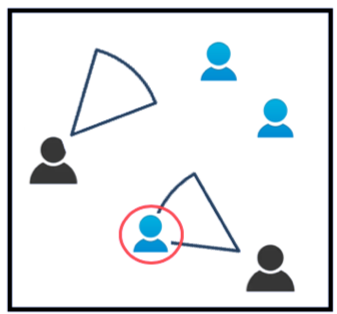
\includegraphics[scale=0.6]{figures/concept_simulation.png}
\caption[シミュレーションの概念図]{シミュレーションの概念図 \label{concept_simulation}}
\end{center}
\end{figure}

\section{知的マルチエージェントモデル}

介護行動は社会系の複雑現象である.私たちが行動を起こす際に,認知症による自己の生理機能への理解が周囲に与える影響を懸念することはあっても,それの繰り返しによって大きな事故につながると理解している人は少ない.しかし,個人レベルでは,手すりに捕まる,他の歩行者に接触しないようにするといった比較的単純なルールに従い行動しているが,それらの個人行動が多種・多量に存在し,相互作用することによって全体としては非常に複雑な現象となる.複雑系を解析する手法の一つとして,マルチエージェント手法がある.しばしば,セルオートマトンが複雑系のシミュレーションに用いられ,セルオートマトンに基づくシミュレーションの研究事例もいくつか存在する.これに対して,本シミュレータでは,人間という知的レベルの高い主体が多数集まり相互作用を起こす介護現象をより精緻に再現するために,情報を知覚し,それを基に自律的に行動を起こす主体を知的エージェント(IntelligentAgent),それを取り巻く世界を環境(Environment)と定義し,シミュレーションの構造はマルチエージェントのフレームワークに基づき構築している.そこで,これを知的マルチエージェントモデルと呼ぶ.

\section{知的エージェント}
図\ref{intelligent_agent}に知的工一ジェントのイメージを示す.知的エージェントは,情報を知覚するセンサーと動作を実行する作用器を持っている.また,エージェント自身の思考プロセスを保持しており,センサーから得られた情報と自分の有する知識と判断基準に基づき自律的に行動を決定し,作用器を通して行動を起こし,環境に働きかける.センサー,作用器,思考は知的エージェントが実際に適用される時点で,問題に応じて定義される.図\ref{agent_modeling}にエージェントと環境の相互作用の様子を模式的に示す.介護者エージェントが自らの行動により環境に影響を与え、その環境によって被介護者エージェントが影響を受けることになる.ある主体の動きによって系全体の動きが規程され,複雑な現象が創発する.

\begin{figure}[htb]
\begin{center}
 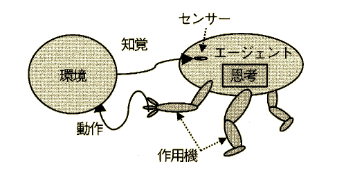
\includegraphics[scale=0.6]{figures/intelligent_agent.png}
 \caption[知的エージェントの模式図]{知的エージェントの模式図 \label{intelligent_agent}}
\end{center}
\end{figure}

\begin{figure}[htb]
\begin{center}
 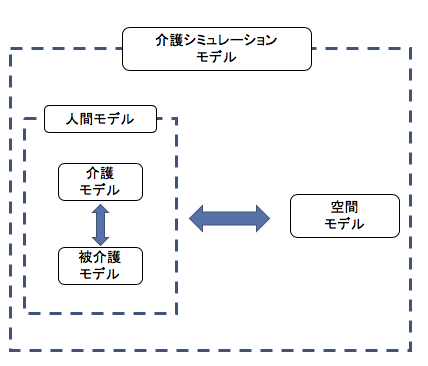
\includegraphics[scale=0.6]{figures/agent_modeling.png}
 \caption[本シミュレーションにおける環境とエージェント]{本シミュレーションにおける環境とエージェント \label{agent_modeling}}
\end{center}
\end{figure}

\section{Social force model}

本研究では,高齢者施設内で介護者が高齢者のトイレ介護のために空間移動するプロセスをモデリングするために,Socialforcemodel(SFM)\cite{SFM}という歩行者モデリング理論を用いる.SFMは,歩行者を2次元の粒子であると仮定し,その粒子に以下の4つの力が働くと仮定するモデルである.

\begin{itemize}
 \item 移動目標に近づく力
 \item 他のエージェントからの斥力
 \item 壁などの環境からの斥力
 \item 魅力的な環境への引力
\end{itemize}

移動目標に近づく引力は,エージェントが当初想定していたコースからはずれてしまった場合に目的地の進行方向へと曲げるように働く力のことであり,他のエージェントや壁などからの斥力は,エージェント間,あるいは壁とエージェント間との距離や,お互いの進行方向から決定される反発的な力のことである.魅力的な環境への引力では,友人やショーウィンドー,高齢者支援施設の中では手すりのような,歩行者にとって近づくことのインセンティブが発生するようなものへの引力のことである.これら4つの力は以下のように数式で表現される.

\begin{equation}
\begin{split}
 F_α(t)=F_α^o(υ_α,υ_α^0e_α)&+\sum_{β}F_αβ(e_α,r_α-r_β)\\
 &+\sum_{B}F_αβ(e_α,r_α-r_B^α)\\
 &+\sum_{i}F_αi(e_α,r_α-r_i,t)
\end{split}
\end{equation}

右辺第一項が移動目標に近づく力,第二項が他のエージェントからの斥力,第三項が壁などの環境からの斥力,第四項が魅力的な環境への引力を表している.各エージェントはタイムステップごとに以上の力を計算して,あらかじめ設定された最大歩行速度を超えないように歩行速度を更新する.

\section{仮想環境}
本シミュレータにおける環境とは,道路構造とそれに含まれる情報一般を指す.道路構造のモデル化はそれ自体が交通流シミュレータの汎用性・拡張性を実現する上で重要な課題である.本シミュレータでは,車は基本的に.申線(レーン)に沿って一次元制こ走行することを仮定する仮想走行レーンモデル101をベースとして道路モデルを構築しており,加えて仮想走行レーンモデルのみでは実現することが難しい大域的な経路探索や,車線変更,追い越し挙動などを実現するために,レーン束オブジェクトとレーン幅という概念を新たに導入した階層型道路モデルを構築した4).本研究では,これに加えて,歩行者を扱うために道路モデルを拡張した.

\subsection{高齢者施設}

現実には,車も歩行者も道路空間を移動するが,それぞれの移動範囲の時空間スケールや従うルールは大きく異なる場合も多い.こうした差異を無視して,道路環境に関して一元的な定義を彳∫うと,シミュレータの汎用性や拡張性を大きく損なうことになる.そこで,歩行者の存在空間を車の存在空問とは独立して定義し,歩彳亅.者空問と車空間のコミュニケーション方式を定義することにより,道路環境を定義することとした,また、今回の開発では,歩行者を扱うための第・ステップとして歩行者工一ジェントの存在範囲を横断歩道に限定した,これは,交通量の多い都市部の幹線道路においては,歩行者が自動車と相彑作用するのは交差点内の横断歩道がほとんどであると考えられるためである,歩行者は図3のような横断歩道エリアの中で行動する,横断歩道はそれぞれ固有の座標空間を持ち,2次元座標を川いてエージェントの位置を表す.横断歩道はエリアの境界に仮想的な滞留スペースを保持しており,歩行者は滞留スペースの中で絶えず発生している,歩行者の,横断歩道の幅方向の初期位骨はランダムに決定する.滞留スベースに存在する歩行者は,該当する信号が青である場合に横断歩道Eに登場する.

\subsection{介護者エージェント}

介護者工一ジェントは2次元の歩行者エリア上に存存するため,方向と速度の制御を行わなければならない.今回は,歩行者の行動モデルとしてSFMを採用した.また歩行者シミュレーションの研究分野において様々なモデル化が検剤されている\cite{ex_pedestrian_simulation_1,ex_pedestrian_simulation_2}.たとえば,磁気モデルを用いると多方向に歩行するエージェントの相互作用を効率的に記述することが可能である.しかし,今回の研究のように横断歩道上での歩行を対象とする場合には,単路を右から左,または左から右に渡る2方向を考慮すれば十分である,また歩行者モデルとしてあまり複雑なモデルを採用すると計算量が増大し交通シミュレータの大規模化が困難であることから,本研究では分岐型2ノ∫向モデルを採用した.以下で歩行者工一ジェントの特徴と挙動について述べる.\\
デルの単純化のために,人体を直径O.45m(成人男子の肩幅)の1[jで近似する.現バージョンのMATESでは高さの情報を解析に用いないため,平面で十分である,さらに,人体円の外側に他人の進入を拒む領域としてパーソナルスペースを設ける,パーソナルスペースとしては様々な形状が提案されているが\cite{ex_personal_space},本研究では1mの直径を持つ円をパーソナルスペースとして定めた.

\subsection{被介護者エージェント}

行者工一ジェントは2次元の歩行者エリア(横断歩道)上に存存するため,方向と速度の制御を行わなければならない.今回は,歩行者の行動モデルとして分岐型2方向モデルtl♪を採用した.文献11)にはより高度なモデルも紹介されている.また歩行者シミュレーションの研究分野において様々なモデル化が検剤されている12・LIItたとえば,磁気モデルを用いると多方向に歩行するエージェントの相互作用を効率的に記述することが可能である.しかし,今回の研究のように横断歩道上での歩行を対象とする場合には,単路を右から左,または左から右に渡る2方向を考慮すれば十分である,また歩行者モデルとしてあまり複雑なモデルを採用すると計算量が増大し交通シミュレータの大規模化が困難であることから,本研究では分岐型2ノ∫向モデルを採用した.以下で歩行者工一ジェントの特徴と挙動について述べる.

%3章
\chapter{提案手法}

本研究で対象とするエージェントシミュレーションの大きな特徴は,介護の対象となる高齢者の運動機能や認知機能の低下に大きなバリエーションがあると同時にも,介護者側にも国家資格をもった介護福祉士から,介護ヘルパー,ボランチィアスタッフまで技能や知識,経験に大きなバリエーションがあることである.そうしたことを念頭に置いた上で,本研究では介護者エージェント,被介護エージェント,環境としての高齢者施設の基本モデリングを検討した.図\ref{concept_simulation}に概念図を示す.黒で示される介護者が、自身が持つ視野の中で水色で示される被介護者を観測する.

\begin{figure}[htb]
\begin{center}
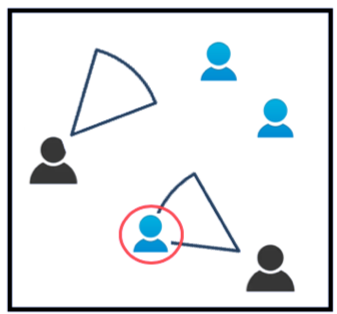
\includegraphics[scale=2.0]{figures/concept_simulation.png}
\caption[シミュレーションの概念図]{シミュレーションの概念図 \label{concept_simulation}}
\end{center}
\end{figure}

\section{知的マルチエージェントモデル}

介護行動は社会系の複雑現象である.私たちが行動を起こす際に,認知症による自己の生理機能への理解が周囲に与える影響を懸念することはあっても,それの繰り返しによって大きな事故につながると理解している人は少ない.しかし,個人レベルでは,手すりに捕まる,他の歩行者に接触しないようにするといった比較的単純なルールに従い行動しているが,それらの個人行動が多種・多量に存在し,相互作用することによって全体としては非常に複雑な現象となる.複雑系を解析する手法の一つとして,マルチエージェント手法がある.しばしば,セルオートマトンが複雑系のシミュレーションに用いられ,セルオートマトンに基づくシミュレーションの研究事例もいくつか存在する.これに対して,本シミュレータでは,人間という知的レベルの高い主体が多数集まり相互作用を起こす介護現象をより精緻に再現するために,情報を知覚し,それを基に自律的に行動を起こす主体を知的エージェント,それを取り巻く世界を環境と定義し,シミュレーションの構造はマルチエージェントのフレームワークに基づき構築している.そこで,これを知的マルチエージェントモデルと呼ぶ.

\subsection{知的エージェントの構築}
図\ref{intelligent_agent}に知的工一ジェントのイメージを示す.知的エージェントは,情報を知覚するセンサーと動作を実行する作用器を持っている.また,エージェント自身の思考プロセスを保持しており,センサーから得られた情報と自分の有する知識と判断基準に基づき自律的に行動を決定し,作用器を通して行動を起こし,環境に働きかける.センサー,作用器,思考は知的エージェントが実際に適用される時点で,問題に応じて定義される.図\ref{agent_modeling}にエージェントと環境の相互作用の様子を模式的に示す.介護者エージェントが自らの行動により環境に影響を与え、その環境によって被介護者エージェントが影響を受けることになる.ある主体の動きによって系全体の動きが規程され,複雑な現象が創発する.

\begin{figure}[htb]
\begin{center}
 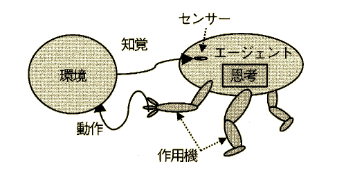
\includegraphics[scale=1.0]{figures/intelligent_agent.png}
 \caption[知的エージェントの模式図]{知的エージェントの模式図 \label{intelligent_agent}}
\end{center}
\end{figure}

\begin{figure}[htb]
\begin{center}
 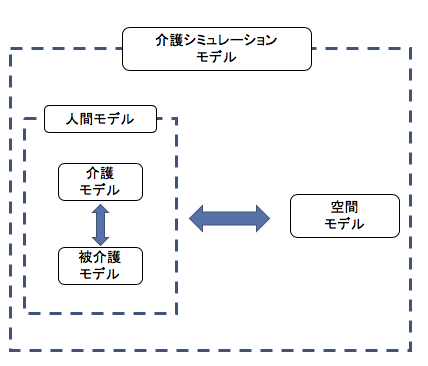
\includegraphics[scale=0.6]{figures/agent_modeling.png}
 \caption[本シミュレーションにおける環境とエージェント]{本シミュレーションにおける環境とエージェント \label{agent_modeling}}
\end{center}
\end{figure}

\subsection{シミュレーションフロー}

本研究におけるシミュレーションの流れの概略図を図\ref{simulation_flow}に示す。まず、高齢者施設、介護者、被介護者といった空間を構成する要素を環境として構成し、その後実際にシミュレーションを開始する。タイムステップごとに、各エージェントの内部状態を変化させ、介護シミュレーションを行っていく。被介護者の場合は、時間経過で尿量を加算し、エージェントごとに設定されている閾値を超えた時点で介護アラートを出す。介護者は、自分の周りで介護アラートが出たタイミングで、自らと最も距離の近い被介護者のもとへの介護に向かう。これを繰り返すことがシミュレーションが進んで行く。

\begin{figure}[htb]
\begin{center}
 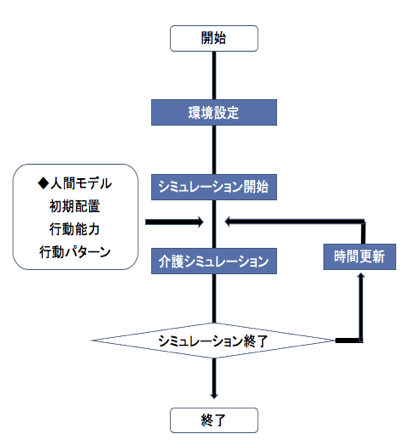
\includegraphics[scale=0.8]{figures/simulation_flow.png}
 \caption[シミュレーションフロー]{シミュレーションフロー \label{simulation_flow}}
\end{center}
\end{figure}

\section{仮想環境}
本シミュレータにおける環境とは,高齢者施設とそこに存在する介護者、被介護者構造を指す.高齢者施設のモデル化はそれ自体が交通流シミュレータの汎用性・拡張性を実現する上で重要な課題である.本シミュレータでは,介護者・被介護者は基本的に.自由移動を行うことができる二次元平面を想定している。

\subsection{高齢者施設}

今回の開発では,高齢者施設を表現するための第1ステップとして,Social Force Modelを利用するため自由に歩行できる連続空間を対象とし、壁に囲まれた移動可能な二次元平面を作成した。
% wallクラスの説明

\subsection{Vectorモデル}

\section{歩行者モデル}

\subsection{経路決定モデル}

\subsection{加速度決定モデル}

本研究では,高齢者施設内で介護者が高齢者のトイレ介護のために空間移動するプロセスをモデリングするために,前述した歩行者シミュレーションの理論の中で,Social force model(SFM)\cite{SFM}を用いる.Social Force Modelは,歩行者を2次元の粒子であると仮定し,その粒子に以下の4つの力が働くと仮定するモデルである.

\begin{itemize}
 \item 移動目標に近づく力
 \item 他のエージェントからの斥力
 \item 壁などの環境からの斥力
 \item 魅力的な環境への引力
\end{itemize}

移動目標に近づく引力は,エージェントが当初想定していたコースからはずれてしまった場合に目的地の進行方向へと曲げるように働く力のことであり,他のエージェントや壁などからの斥力は,エージェント間,あるいは壁とエージェント間との距離や,お互いの進行方向から決定される反発的な力のことである.魅力的な環境への引力では,友人やショーウィンドー,高齢者支援施設の中では手すりのような,歩行者にとって近づくことのインセンティブが発生するようなものへの引力のことである.

\subsection{介護者エージェント}

介護者工一ジェントは2次元の高齢者施設に存存するため,方向と速度の制御を行わなければならない.今回は,歩行者の行動モデルとしてSocial Force Modelを採用した.歩行者シミュレーションの研究分野においては、様々なモデル化が検剤されている\cite{ex_pedestrian_simulation_1,ex_pedestrian_simulation_2}.たとえば,磁気モデルを用いると多方向に歩行するエージェントの相互作用を効率的に記述することが可能である.しかし,今回の研究のように閉二次元平面での歩行を対象とする場合には,部屋の中を目的地に対してどう動いて行くかを単純に記述するモデルで十分である.また歩行者モデルとしてあまり複雑なモデルを採用すると計算量が増大しシミュレータの大規模化が困難であることから,本研究ではSocial Force Modelを採用した.以下で歩行者工一ジェントの特徴と挙動について述べる.

\subsubsection{介護プロフェッショナル段位制度}

\subsubsection{介護ステータス}

\subsection{被介護者エージェント}

被介護者エージェントについては、介護者エージェントと同様にSocial Force Modelを軸に、歩行者エージェントを作成し、それに加えてエージェントの状態によって時系列的に発生する要介護行動を実装した.高齢者の排尿に関する実態研究 \cite{micturition} によると、排尿障害症状を自覚している人は男子が38%、女子が23%と高い水準にあり、男子では排尿困難症状が多く、女子では頻尿を訴える例が多かった。また明らかな尿失禁を抱えているのにも関わらず、その存在を知られたくないという心理が半数以上の人に認められたことも挙げられている。これらから、実際にトイレに行きたいと思っているかどうかの認知についてと、トイレで正常に排尿を行えるのかどうかといった機能について、被介護者のバリエーションを設けることとした.

\subsubsection{要介護度}

\subsection{内部変数}
%トイレに行った回数,我慢した秒数,膀胱のキャパシティ

\subsubsection{介護アラート}

\subsection{介護ペア選択アルゴリズム}

上述のように、被介護者がアラートを発した時にどの介護士とマッチングさせるのかというのがシミュレーション上必要になる。本研究では、各タイムステップごとにある被介護者がアラートを出した時点で、その被介護者と介護可能な介護士との距離を計算し、ペアになりうる介護士と被介護者のペア候補配列を作成していき、その中で全探索を行うことで、最も距離の近いペアを作成して行くこととする。

% 4章
\chapter{結論}

\section{本研究のまとめ}

本研究では,介護支援施設の主体(ここでは研究の第一段階として介護者,被介護者のみに着目する)を,能動的に自分自身で情報を集めて行動する主体性,すなわち自律性を持つ知的エージェントとしてモデル化し,多数の知的工一ジェントを仮想的な遭路環境上で相互作用させることによって,介護環境をシミュレーションする,知的マルチエージェントモデルに基づくシミュレータを構築した.本論文では,はじめに,本シミュレータに組み込まれた知的マルチエージェントモデルの理論及び実装法について述べた.次に,被介護者の状態によっていくつかの異なる環境を構成し、将来医療技術が発達して行くとどれほどのインパクトをもたらすのかについて,かなり艮好な数値を示すことを確認した.

\section{今後の展望}
本シミュレータについて,絶対値レベルでの定量的な現状再現性については,信頼できる介護施設データが足りておらず,理論値を元に実測値と比較することでモデルの有用性について検証して行く必要がある.

% 介護士の業務量について定量的に評価できる指標の導入も行いたい.

% 5章
\chapter{数値実験}

研究で新たに実装した歩行者工一ジェントおよび介護シミュレーションの定量的な評価性能を検証するために,シミュレーション実験を行った.
この章では,実験で用いた環境設定と,実験結果をどのような評価指標で判断したか,またその結果と考察についてまとめている.

\section{実験条件}

今回の実験では介護環境として,図\ref{environment}に示すように,15m四方の二次元平面と,排泄場所としてのトイレをその上部に設置した.

\begin{figure}[htb]
\begin{center}
 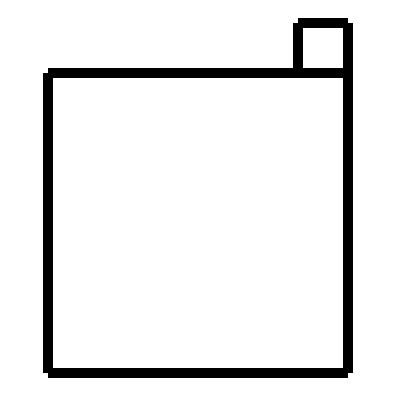
\includegraphics[scale=0.5]{figures/environment.png}
 \caption[実験環境]{実験環境 \label{environment}}
\end{center}
\end{figure}

この環境の中で,介護者と被介護者の可視化をおこなっていく.今回の実験では,介護における技術を導入した際に,それが介護環境にどのようなインパクトをあたえるのかについて検証を行うことが目的なので,介護者の数は1人,被介護者の数は16人と設定し,比較的大きい施設を対象とした.第4章で述べた適切なタイミングで介護要望フラグをたてる被介護者,早いタイミングで介護要望フラグをたてる被介護者の被介護者,遅いタイミングで介護要望フラグをたてる被介護者の被介護者の3種類のエージェントが,介護施設内の自由時間である2時間の間にいかなる回数にわたって排泄介助を行うことが必要か,またその介助は本当に必要であったのかということを確かめる実験をおこなう.3種類の被介護エージェントを\ref{experiment}のように組み合わせた6パターンにおいて,相互作用を確認し,それを本章で示す評価指標で評価する.

\begin{figure}[htb]
\begin{center}
 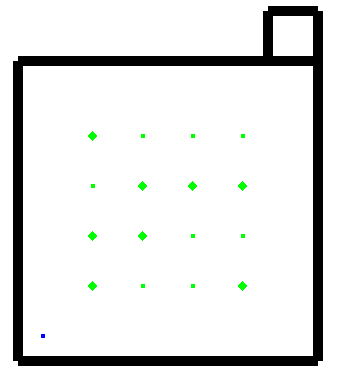
\includegraphics[scale=0.5]{figures/health_urinate.png}
 \caption[適切なタイミングで介護要望フラグをたてる被介護者と遅いタイミングで介護要望フラグをたてる被介護者の場合の可視化]{適切なタイミングで介護要望フラグをたてる被介護者と遅いタイミングで介護要望フラグをたてる被介護者の場合の可視化 \label{health_urinate}}
\end{center}
\end{figure}

\begin{figure}[htb]
\begin{center}
 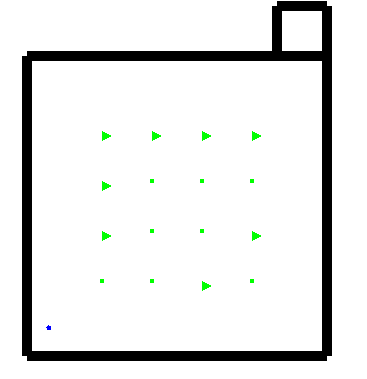
\includegraphics[scale=0.5]{figures/health_frequently_urinate_v1.png}
 \caption[適切なタイミングで介護要望フラグをたてる被介護者と早いタイミングで介護要望フラグをたてる被介護者の場合の可視化]{適切なタイミングで介護要望フラグをたてる被介護者と早いタイミングで介護要望フラグをたてる被介護者の場合の可視化 \label{health_frequently_urinate_v1}}
\end{center}
\end{figure}

\begin{figure}[htb]
\begin{center}
 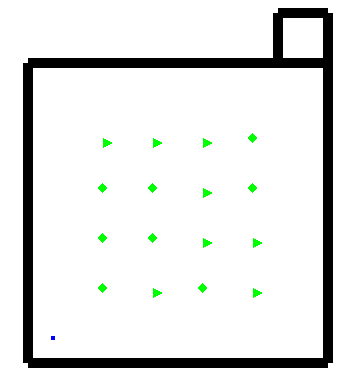
\includegraphics[scale=0.5]{figures/dementia_urinate_v1.png}
 \caption[遅いタイミングで介護要望フラグをたてる被介護者と早いタイミングで介護要望フラグをたてる被介護者の場合の可視化]{遅いタイミングで介護要望フラグをたてる被介護者と早いタイミングで介護要望フラグをたてる被介護者の場合の可視化 \label{dementia_urinate_v1}}
\end{center}
\end{figure}

\begin{table}[htb]
  \caption[実験条件]{実験条件}
  \label{experiment}
  \centering
  \begin{tabular}{r|c|c|c|c|c|c|c}
     & Case1 & Case2 & Case3 & Case4 & Case5 & Case6 & Case7 \\ \hline
    適切 & 100% & 0% & 0% & 50% & 50% & 0% & 33% \\
    早い & 0% & 100% & 0% & 50% & 0% & 50% & 33% \\
    遅い & 0% & 0% & 100% & 0% & 50% & 50% & 33% \\
    \end{tabular}
\end{table}

表\ref{experiment}に示したように,Case1は、健常の被介護者(技術の補助を受けた被介護者)が100%の状態,Case2は早いタイミングで介護要望フラグをたてる被介護者の被介護者が100%の状態,Case3は遅いタイミングで介護要望フラグをたてる被介護者の被介護者が100%の状態,Case4は、健常の被介護者(技術の補助を受けた被介護者)と早いタイミングで介護要望フラグをたてる被介護者の被介護者が50%ずつの状態,Case5は健常の被介護者(技術の補助を受けた被介護者)と遅いタイミングで介護要望フラグをたてる被介護者の被介護者が50%ずつの状態,Case6は早いタイミングで介護要望フラグをたてる被介護者の被介護者と遅いタイミングで介護要望フラグをたてる被介護者の被介護者が50%ずつの状態である.なお,Case7に関しては,16人という設定上同じ設定で3等分できなかったので,(5,5,6),(5,6,5),(6,5,5)の3回の平均値をとることにした.なお,Case1は,適切なタイミングで介護要望フラグを立てる設定であり,被介護者に適切なサポートが入っている状態であるので,実験結果はCase1とそれぞれを比較することで技術によるサポートのインパクトを評価することができる.

\section{介護挙動の基本的な検証}

本シミュレータが現実を反映できているのかについて,簡単な検証を行った.介護アラートを出す条件を,適切なタイミングで介護要望フラグをたてる被介護者の場合は100ml以上になった時点,早いタイミングで介護要望フラグをたてる被介護者の場合は75ml以上になった時点,遅いタイミングで介護要望フラグをたてる被介護者の場合は150ml以上で介護アラートを発する設定にし,2時間シミュレータを回した.その結果,適切なタイミングで介護要望フラグをたてる被介護者の場合は,2時間に1回トイレに行くという結果を得ることができた.これは実際のデータと比較しても整合性のある値となった.この結果を表\ref{number_of_urination}に示す.なお,実験では16人の被介護者が存在するので実際は数値を16で割った数字が一人当たりの回数となっている.

\begin{table}[htb]
  \caption[被介護者ごとの排尿回数]{被介護者ごとの排尿回数}
  \label{number_of_urination}
  \centering
  \begin{tabular}{r|c|c|c}
     & 適切なタイミング & 早いタイミング & 遅いタイミング \\ \hline
    一回目 & 15 & 21 & 6 \\
    二回目 & 15 & 22 & 5 \\
    三回目 & 16 & 26 & 5 \\
  \end{tabular}
\end{table}

\section{評価指標}

本研究の目的は,疾患のある被介護者,すなわち現状介護者の負担増の原因となっており,被介護者自身も自らの排泄が負担となっているようなケースにおいて,技術の導入を行うことでどれだけの効果が得られるのかを可視化するというものである.そこで,評価指標として,介護者の負担を示す指標として,行った介護回数,被介護者が強いられた負担を示す指標として,排泄に行くべきである尿量の状態,あるいは自身が排泄に行きたいと感じている状態から実際に排泄を行うまでの時間を計測し,それを総我慢時間とする.

\section{結果および考察}

図\ref{result_v1}に,介護者・被介護者の割合をCase1からCase7までそれぞれ変化させた場合のシミュレーション結果(10回の試行の平均値)を示す.表\ref{relative_error}に,それぞれの具体的な数値とCase1に対する相対誤差を示した.次に表\ref{number_of_care}に,Caseごとの介護回数とCase1に対する相対誤差を示した.

\begin{figure}[htb]
\begin{center}
 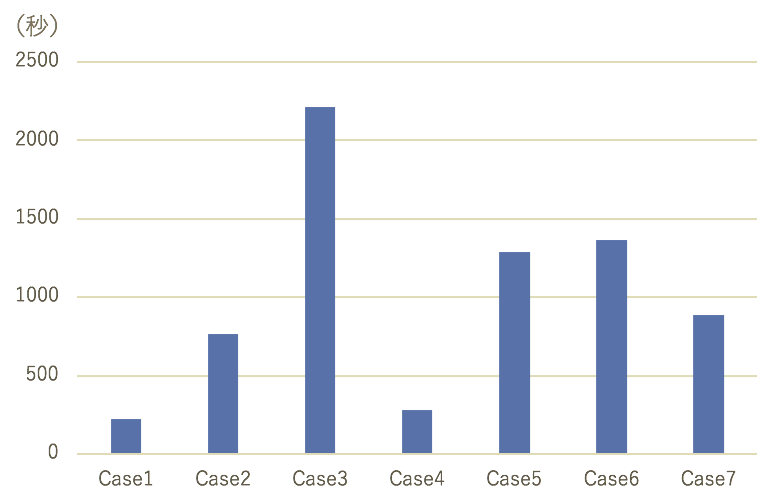
\includegraphics[scale=0.5]{figures/result_v1}
 \caption[実験結果]{実験結果 \label{result_v1}}
\end{center}
\end{figure}

\begin{table}[htb]
  \caption[Caseごとの我慢時間]{Caseごとの我慢時間}
  \label{relative_error}
  \centering
  \begin{tabular}{r|c|c|c|c|c|c|c}
     & Case1 & Case2 & Case3 & Case4 & Case5 & Case6 & Case7 \\ \hline
    我慢時間 & 220.1 & 764.0 & 2213.5 & 278.4 & 1285.9 & 1363.7 & 884.3 \\
    相対誤差 & & 2.47 & 9.05 & 0.26 & 4.84 & 5.19 & 3.02 \\
    \end{tabular}
\end{table}


\begin{table}[htb]
  \caption[Caseごとの介護回数]{Caseごとの介護回数}
  \label{number_of_care}
  \centering
  \begin{tabular}{r|c|c|c|c|c|c|c}
     & case1 & Case2 & Case3 & Case4 & Case5 & Case6 & Case7\\ \hline
    介護回数 & 15-16 & 21-26 & 5-6 & 19-21 & 9-10 & 16-17 & 15-18\\
    相対誤差 & & 0.50 & -0.65 & 0.31 & -0.37 & 0.07 & 0.09 \\
    \end{tabular}
\end{table}

Case2については,過剰介護が問題であると考えられる.適切なタイミングで介護要望フラグをたてる被介護者の場合と比べ,50%以上も介護士の労働力に悪影響を与えているといえる.早いタイミングで介護要望フラグをたてる被介護者の場合は,単純にトイレに行かないという選択肢を現場で取ることができないので,おむつなどで現場では対応していると考えられる.しかしおむつは,被介護者の自立意識を妨げるツールであるので,その使用については注意が必要である.どのタイミングでおむつをつけることを決め,どの時点でつけることをやめるのか,その意思決定基準はブラックボックスになっている.しかしCase4の結果を見ると,被介護者の我慢時間がCase1との相対誤差が小さいことに加えて,実際の介護回数も相対誤差0.31に留まっている.すなわちシミュレーションによって,高齢者施設がどういった状態の被介護者を受け入れるか,あるいはどの被介護者同士を同じ部屋に入れ,一人の被介護者に対応させるのかといった人事配置について示唆を得ることができることを示している.

Case3の総我慢時間が,もっとも高いものとなっているが,これは被介護者が本来なら排泄に向かうべき尿量であるのにも関わらず,無意識のうちに我慢をしてしまい,介護者にアラートを出した時点ですでにかなりの時間を待ち時間として計測してしまっていることが原因であることが考えられる.逆に言えば,技術を導入することでCase1の状態へと環境を変えることで,被介護者の我慢時間を述べ約2000秒も短縮することができる.

Case5では,数値上は相対誤差がかなり少ないように見えるが,実際は適切なタイミングで介護要望フラグをたてる被介護者と遅いタイミングで介護要望フラグをたてる被介護者の被介護者の間の待ち時間の差が大きく,適切なタイミングで介護要望フラグをたてる被介護者の割合が減ったことで,適切なタイミングで介護要望フラグをたてる被介護者がアラートを出した際にすぐ介護してもらえたということがあげられる.実際の現場では,被介護者の要介護によって,どの介護者がつくべきかということが事前情報として与えられているため,このような複雑な状況にも対応していけるような環境をつくっているという示唆を得ることができる.今後の検討課題として,そういった事前情報の有無によって,どの介護者と被介護者をマッチングさせるのかということが挙げられる.具体的にどのような事前情報に基づいて意思決定が行われているのか今後の調査課題である.

Case6は我慢時間こそ多いものの,介護回数についてはCase1とそれほど違いが出ていない.しかし,これも早いタイミングで介護要望フラグをたてる被介護者の被介護者に対する介護が多く,遅いタイミングで介護要望フラグをたてる被介護者の被介護者に対する介護回数が少ないので,合計回数が相殺してCase1と近い値が出てしまったためである.

Case7について,介護回数では早いタイミングと遅いタイミングの被介護者同士が打ち消しあうので,Case1と差が出ないことは直感的に正しい.我慢時間をCase6と比較した際にも,約2/3倍であり適切なタイミングではない被介護者の数におおむね比例している.

%
%% 後付け
\backmatter
\chapter{謝辞}

指導教員であり,本研究の機会を与えていただいた,吉村教授に感謝いたします.研究への姿勢や考え方など,右も左もわからなかった私に一から丁寧に教えていただきました.また,就職活動でもお気遣いいただき,本当に感謝しております.研究を通じて先生に教えていただいた,物事を構造的に捉え,仮説を持って取り組む姿勢は,授業では決して得られない貴重な学びになりました.先生から学んだ仮説思考とも言える考え方は,研究の領域に留まらず,人生においてとても重要なものであると確信しております.今回私は,これまで研究室にはなかった医療というフィールドでの研究を0から始めたわけですが,このようなチャレンジングな機会を与えていただいたこと,また研究内容が社会的意義のあるものだと感じたまま研究に取り組めたことは自分の修士課程にとってとても大きなことでした.本研究での経験や学びを忘れず,社会のために生かして参りたいと存じます.ゼミのディスカッションや研究打ち合わせでは,私に合わせて理解のしやすい説明も織り交ぜながら,医療現場について,研究発表について,教えていただきました.先生とのミーティングは,医療業界全体が抱えるマクロ的な課題をはじめとして,私の母親の例だと,といったようにミクロ的な物事の捉えかた,縦横無尽に課題を探索していく思考の柔軟さに圧倒されることが多く,非常に学びの多い時間でした.とても忙しいはずなのに何冊も本を読み,貪欲に知識を蓄えていく姿勢は,私も今後死ぬまで持ち続けていきたいと心から感じております.これからは,吉村研究室の名に恥じない,社会に価値を提供できる人間になり,吉村研究室の卒業生として世界に名を馳せるよう精進いたします.また,いつも単位のことを気にかけてくださり,本当に感謝してもしきれません.約二年間,大変お世話になりました.ありがとうございました.\\
\\
\quad 藤井講師には,社会系勉強会にて相談に乗っていただき,研究の進め方について,多岐にわたるご指導,ご助言をいただきました.資料を作成する際にも,研究に取り組む際にも,常に一貫した考えで,目的意識を持って論理的に考えるという姿勢を学ばせていただきました.ご多忙の中,勉強会にてアドバイスをいただき,考察を深めたこ日々は大変貴重で,充実した日々でありました.研究室に入った当初,富士樹海に迷い込んだ子羊だった私が,道を踏み外すことなく,本研究をここまで勧められたのは,藤井先生という北極星が強く光り輝き,導いてくださったからに他なりません.些細なことでも,いつも心よく相談に乗ってくださり学生に親身になってくださる姿勢は私含め多くの学生の心の支えになっていたと思います.私が修士一年の頃,よくゼミでは活発に議論が行われ,今はなきY先生と学生が口論を始めた時にはこの研究室に入って正解だったのかと,いまにも逃げ出したほうがいいのではないかと悪魔の囁きが心の中で誘惑をしていたのですが,そのような緊急事態にもまるで慌てることなく何もなかったことのようにそれを眺める藤井先生の器量の大きい姿が今でも忘れられません.二年間本当にありがとうございました.\\
\\
\quad 内田さんは,自分の研究について一番アドバイスをくださり,実際にコードまで見ていただいた感謝しても仕切れない存在です.研究のけの字も,交通シミュレーションのこの字も,知らない私に一からなんでも優しく教えていただきました.特に私が一週間かかっても解決できなかった問題をほんの一時間ほどで解決した際には,内田さんの後ろからまばゆいばかりの光がさしこみ,菩薩かのような貫禄まで漂っていたことを覚えております.ゼミや社会系勉強会での内田さんの指摘は毎度とても鋭く,ロジックの抜け漏れには誰よりも早く気づき,それを指摘する姿は,研究者でありながらコンサルティングファームのパートナーかのような頭の回転を彷彿とさせておりました.特に私が研究室に入ったばかりの頃,自らの発表資料を先輩の資料をもとに作成した際に,これ資料作成者違う人になってるけど,本当にあなたが作ったんですか?と言われた際には,冷や汗が止まらず,このまま隕石でも落ちて地球がなくなってしまわないかなと感じていたことは,生涯忘れられない思い出となりました.自分の作品には責任を持って,自分で書き上げるという当たり前のことを学ぶことができました.本当にありがとうございました.\\
\\
\quad 阿部さんは,社会系勉強会をはじめとしてCDの発表相手にもなっていただき,自分としては一番距離の近い兄貴のような存在でした.まるで,きびだんごを持たない生まれたての桃太郎のような私に無償でついてきてくださる虎のような存在でした.時にはパワーポイントの使い方を,時には資料のスキャンの方法を,時にはポスターを額縁に入れる方法を教えてくださり,鬼を倒すがごとく研究を進めることができました.勉強会の際には,他の先生方が厳しい質問をしている一方で,阿部さんはコメントと質問を織り交ぜて,学生がしっかり頭を使って答えることができるようにいつも誘導してくださっていて,優しさの溢れる質疑となっていたことが思い出されます.学生が阿部さんの質問を理解できなかった時には,阿部さんが再度「要するに」といって補足してくださるのですが,話している間にどんどん優しさが溢れて行って,最終的にはほとんど答えを言ってしまっていて、全然要せていないことも,阿部さんの人間力と優しさからくるものだなと日々感銘しておりました.私も阿部さんのように知性だけでなく人類を包み込むような優しさと,まるで母親が息子に向けるかのような暖かい笑顔を身につけることのできる人間になりたいと思います.二年間ありがとうございました.\\
\\

%研究室の皆様

%同期

%井上さん
 % 謝辞
\begin{thebibliography}{99}
 \bibitem{ex_kousei_v1} 厚生労働省, 平成28年版厚生労働白書(2016)
 \bibitem{SFM} D.HELBING, P.MOLNAR:Social force model for pedestrian dynamics, Physical Review E 41, 4282,(1995)
 \bibitem{ex_pedestrian_simulation_1} 岡崎甚幸:建築空間における歩行のためのシミュレーションモデルの研究その1 磁気モデルの応用による歩行モデル,目本建築学会論文服告集,2S3,111/ll7(1979)
 \bibitem{ex_pedestrian_simulation_2} Kurdi Teknomo、Groria P.Gerilla:Sensitivity Analysis And Validation of a Multi−Agents Pedestrian Model,Journal of the Eastern Asia Society for Transportation Studies,6,198/213(2005)
 \bibitem{ex_personal_space} 渋谷昌三:パーソナル・スペースの形態に閏する考察,山梨医科大学紀要,2,41/49(1985)
 \bibitem{micturition} 安藤正夫:高齢者における排尿障害の実態について,日本泌尿器科学会誌,82,560/564(1991)
 % \bibitem{mates} MATESの引用
\end{thebibliography}
 % 参考文献
%
\end{document}
